\chapter{Multiprocessor systems}

\section{Supercomputing}

Supercomputing represents the high performance segment of the overall computing
market. This segment has traditionally been driven by grand challenge problems
in science and engineering. This is still the situation, although new areas and
new applications are constantly being added to the list of problems where
supercomputing is necessary (or at least highly desirable).

A strong motivation for using supercomputing is the possibility of performing
larger and more realistic simulations, e.g., by solving more detailed
mathematical models in science and engineering. Hence, the design of the largest
computing systems have traditionally be driven by challenges in science and
engineering.

About 30--40 years ago, supercomputers were typically specially designed vector
processors capable of performing operations on vector data. A single instruction
could operate on multiple data elements (vectors) at once, and the hardware
comprised custom-made chips. Because of the low production volume and the costly
development effort, each supercomputer was very expensive.

Supercomputers in the 80s and 90s also used fast, expensive, custom-made chips,
and combined a few of these in a multiprocess context. However, starting in the
late 80s, microprocessor-based supercomputers became more and more popular.
These systems were also called \emph{massively parallel processors} (MPPs)
because they used many more processors than traditional vector supercomputers.
The advantage of the microprocessor-based supercomputers was the use of
standard, off-the-shelf microprocessors instead of using costly, custom-made
chips. The supercomputer market today is dominated by MPP systems. A
supercomputer system typically combines thousands of processors. Some of the
largest systems comprise hundreds of thousands of processors.

Supercomputing is very resource demanding in terms of floating point operations,
memory and storage requirement, as well as visualization capabilities. Thus,
some of the important challenges related to the development and use of a
multiprocessor system concern:
\begin{enumerate}
\item communication between the processors \\
(network topology, memory access, programming models);
\item development of suitable computational methods or algorithms \\
(e.g., domain decomposition algorithms);
\item scalability (both in terms of hardware and algorithms);
\item handling of large volumes of data (storage and visualization).
\end{enumerate}

We add some additional remarks regarding scalability. Let $T_P$ be the time to
solve a given problem on $P$ processors, where time refers to wall clock time.
We define the speedup, $S_P$, as
\begin{align}
  S_P = \frac{T_1}{T_P},
  \label{multi:speedup}
\end{align}
i.e. as the ratio between the solution time on a single processor divided by the
solution time on $P$ processors. Ideally, we would like $S_P$ to be equal to
$P$, implying the $P$ processors should be able to solve the problem $P$ times
as fast as a single processor. A more realistic situation is depicted in
\autoref{fig:scalability}: for small systems (i.e. when $P$ is small), we
typically get good speedup for a fixed problem. As more processors are added,
the computational task per processor is reduced, while the communication
overhead between the processors typically increases. Hence, after a certain
number of processors, it does not pay off to add more processors.

Note that the above situation gives a too pessimistic view of supercomputing.
The assumption about a fixed problem size is typically not correct. With the
availability of larger computing systems, the problem size is typically also
increased. Many problems solved on large systems are of a size that cannot be
solved in a single processor context, either because of the storage requirement,
because of the computational cost, or both. From this view point, the definition
of speedup in \eqref{multi:speedup} must be used with some care.

\begin{figure}
  \centering
  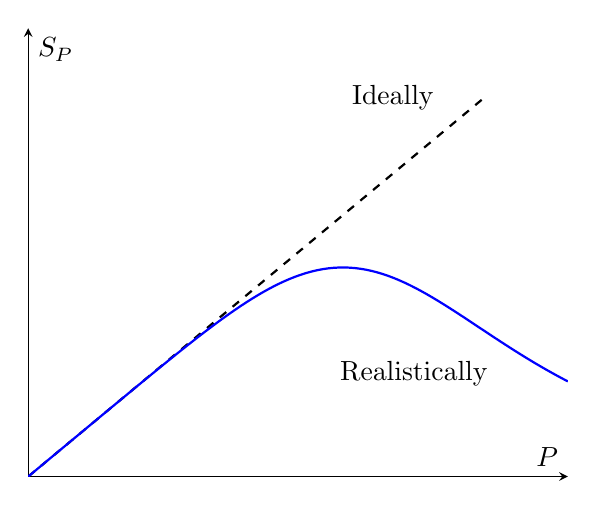
\begin{tikzpicture}
    \begin{axis}[
      xmin=0,
      xmax=1.3,
      ymin=0,
      ymax=1.3,
      axis lines=middle,
      ticks=none,
      xlabel={$P$},
      ylabel={$S_P$},
      ]
      \addplot[dashed, thick, domain=0:1.1, samples=100]{x};
      \addplot[blue, thick, domain=0:1.3, samples=100]{x/(1+x^5)};
      \node at (axis cs:1.0,1.1) [anchor=east] {Ideally};
      \node at (axis cs:1.13,0.3) [anchor=east] {Realistically};
    \end{axis}
  \end{tikzpicture}
  \caption{Ideal speedup ($S_P = P$) and realistic speedup.}
  \label{fig:scalability}
\end{figure}

Finally, a couple of important reminders: when working in a multiprocessor
environment, the single-processor performance is still of utmost importance. In
particular we recall some of the possibilities of parallelism within a single
processor: bit-level, instruction-level, pipelining, and superscalar
capabilities (or multiple floating point units).

\section{Organization of multiprocessor systems}

According to Almasi and Gottlieb (1989), a parallel computer is a collection of
processing elements which communicate and cooperate to solve a problem fast.
This definition raises some immediate questions:
\begin{itemize}
\item How many processing elements should we use?
\item How should the processing elements communicate?
\item Will the parallel computer be scalable?
\item How powerful should a processor be?
\item What about programming?
\end{itemize}

\Autoref{fig:multiprocess1, fig:multiprocess2} show two examples of
organizations. In \autoref{fig:multiprocess1} each processor has a local cache
and can access memory modules via some type of interconnect. In this case, all
the memory modules can be accessed directly by all the processors. This
organization is referred to as \emph{global} or \emph{shared memory access}. In
\autoref{fig:multiprocess2} each processor has local memory and can only access
information in other memory modules via an interconnecting network. This
organization is referred to as \emph{distributed memory access}. Each
organization has its strengths and weaknesses. We will return to some of these
issues later.

\begin{figure}
  \centering
  \begin{tikzpicture}[scale=0.5]
  \foreach \i in {0,4,8}
  {
    \draw[darkblue, fill=cadet, thick] (\i,10) rectangle (\i+2,7);
    \draw[darkblue, very thin, dashed] (\i,8.5) -- (\i+2,8.5);
    \draw[darkblue, fill=cadet, thick] (\i,3) rectangle (\i+2,1.5);
    \draw[darkblue, thick] (\i+1,7) -- (\i+1,6);
    \draw[darkblue, thick] (\i+1,3) -- (\i+1,4);
    \node at (\i+1,9.25) {P};
    \node at (\i+1,7.75) {\$};
    \node at (\i+1,2.25) {M};
  }
  \draw[darkblue, thick] (0,6) rectangle (10,4);
  \node at (5,5) {Interconnect};
\end{tikzpicture}

  \caption{A parallel computer with global memory access.}
  \label{fig:multiprocess1}
\end{figure}

\begin{figure}
  \centering
  \begin{tikzpicture}[scale=0.5]
  \foreach \i in {0,4,8}
  {
    \draw[darkblue, fill=cadet, thick] (\i,10) rectangle (\i+2,7);
    \draw[darkblue, very thin, dashed] (\i,8.5) -- (\i+2,8.5);
    \draw[darkblue, fill=cadet, thick] (\i,6) rectangle (\i+2,4.5);
    \draw[darkblue, thick] (\i+1,7) -- (\i+1,6);
    \draw[darkblue, thick] (\i+1,3.5) -- (\i+1,4.5);
    \node at (\i+1,9.25) {P};
    \node at (\i+1,7.75) {\$};
    \node at (\i+1,5.25) {M};
  }
  \draw[darkblue, thick] (0,1.5) rectangle (10,3.5);
  \node at (5,2.5) {Interconnect};
\end{tikzpicture}

  \caption{A parallel computer with distributed memory access.}
  \label{fig:multiprocess2}
\end{figure}

\subsection{Uniform memory access}

There are several ways to achieve global memory access. One type of systems is
referred to as SMP: \emph{Symmetric Multi-Processor}. This is a configuration
where all the memory locations are ``equidistant'' in the sense that the memory
access time is the same.

An example of an SMP is a bus-based organization; see
\autoref{fig:bus_organization}. This system has a broadcast interconnect similar
to ethernet. It is inexpensive and it is easy to add processors. The
disadvantage with a bus organization is the very limited scalability, which is
due to the fact that the aggregate bandwidth is fixed. The use of caches could
potentially alleviate some of this problem, but then the question of how to
achieve cache coherency (or consistency) arises.

\begin{figure}
  \centering
  \begin{tikzpicture}[scale=0.5]
    \foreach \i in {-1,3}
    {
      \draw[darkblue, fill=cadet, thick] (\i,4) rectangle (\i+2,1);
      \draw[darkblue, very thin, dashed] (\i,2.5) -- (\i+2,2.5);
      \draw[darkblue, thick] (\i+1,1) -- (\i+1,0);
      \node at (\i+1,3.25) {P};
      \node at (\i+1,1.75) {\$};
    }
    \foreach \i in {7,11}
    {
      \draw[darkblue, fill=cadet, thick] (\i,2.5) rectangle (\i+2,1);
      \draw[darkblue, thick] (\i+1,1) -- (\i+1,0);
      \node at (\i+1,1.75) {I/O};
    }
    \foreach \i in {1,5,9}
    {
      \draw[darkblue, fill=cadet, thick] (\i,-2.5) rectangle (\i+2,-1);
      \draw[darkblue, thick] (\i+1,-1) -- (\i+1,0);
      \node at (\i+1,-1.75) {M};
    }
    \draw[red, very thick, <->] (-3,0) -- (15,0);
  \end{tikzpicture}
  \caption{
    A bus-based organization. The global memory is accessible to each processor.
  }
  \label{fig:bus_organization}
\end{figure}

Another example of an SMP is a crossbar or a switch-based organization. Similar
to a bus-based system, cache coherency is needed (e.g. via broadcast). A
crossbar has a better scalability than a bus organization. The aggregate
bandwidth is increased, but adding a processor becomes more and more expensive
as the system size grows (because the number of parts increases).

\begin{figure}
  \centering
  \begin{tikzpicture}[scale=0.5]
  \foreach \i in {0,3,6,9}
  {
    \draw[red, very thick] (0,\i) -- (11,\i);
    \draw[red, very thick] (\i,0) -- (\i,11);

    \draw[darkblue, fill=cadet, thick] (11,\i+.75) rectangle (13,\i-.75);
    \node at (12,\i) {M};
  }

  \foreach \i in {0,3}
  {
    \draw[darkblue, fill=cadet, thick] (\i-1,14) rectangle (\i+1,11);
    \draw[darkblue, very thin, dashed] (\i-1,12.5) -- (\i+1,12.5);
    \node at (\i,13.25) {P};
    \node at (\i,11.75) {\$};
  }

  \foreach \i in {6,9}
  {
    \draw[darkblue, fill=cadet, thick] (\i-1,12.5) rectangle (\i+1,11);
    \node at (\i,11.75) {I/O};
  }
\end{tikzpicture}

  \caption{
    A crossbar interconnect. The global memory is accessible to each processor.
  }
  \label{fig:crossbar}
\end{figure}

In summary, there is a scalability problem with the interconnect both with a bus
organization and with a crossbar. In the case of the bus, the scalability issue
is due to the fixed aggregate bandwidth; in the case of the crossbar, the
scalability relates to the cost. An example of a compromise between these two
issues is the multistage interconnect; see
\autoref{fig:multistage_interconnect}.

\begin{figure}
  \centering
  \begin{tikzpicture}[scale=0.5]
    \foreach \i in {0,4,8,12}
    {
      \draw[darkblue, fill=cadet, thick] (\i-1,0) rectangle (\i+1,1.5);
      \draw[darkblue, thick] (\i,1.5) -- (\i,2.5);
      \draw[darkblue, thick] (\i,8.5) -- (\i,9.5);
      \node at (\i,0.75) {M};
    }

    \foreach \i in {0,4}
    {
      \draw[darkblue, fill=cadet, thick] (\i-1,12.5) rectangle (\i+1,9.5);
      \draw[darkblue, very thin, dashed] (\i-1,11) -- (\i+1,11);
      \node at (\i,11.75) {P};
      \node at (\i,10.25) {\$};
    }

    \foreach \i in {8, 12}
    {
      \draw[darkblue, fill=cadet, thick] (\i-1,9.5) rectangle (\i+1,11);
      \node at (\i,10.25) {I/O};
    }

    \foreach \i in {2, 10}
    {
      \foreach \j in {3.5, 7.5}
      {
        \draw[darkblue, thick] (\i-3,\j-1) rectangle (\i+3,\j+1);
        \node at (\i,\j) {Interconnect};
      }
    }

    \draw[darkblue, thick] (0,4.5) -- (0,6.5);
    \draw[darkblue, thick] (12,4.5) -- (12,6.5);
    \draw[darkblue, thick] (4,4.5) -- (8,6.5);
    \draw[darkblue, thick] (8,4.5) -- (4,6.5);
  \end{tikzpicture}
  \caption{
    A multi-stage interconnect. The global memory is accessible to each processor.
  }
  \label{fig:multistage_interconnect}
\end{figure}

\subsection{Non-uniform memory access}

An alternative to an SMP-organization is a NUMA-organization (\emph{Non-Uniform
Memory Access}); see \autoref{fig:NUMA}. The last supercomputers at NTNU all
represent examples of this type of organization.

\begin{figure}
  \centering
  \begin{tikzpicture}[scale=0.5]
    \foreach \i in {3, 10}
    {
      \draw[darkblue, thick] (\i+1,-2) -- (\i+1,0);
      \draw[darkblue, thick] (\i,-2) -- (\i+2,-2);

      \draw[darkblue, fill=cadet, thick] (\i-2,-2.75) rectangle (\i,-1.25);
      \node at (\i-1,-2) {M};

      \draw[darkblue, fill=cadet, thick] (\i+2,-1.25) rectangle (\i+4,-4.25);
      \draw[darkblue, very thin, dashed] (\i+2,-2.75) -- (\i+4,-2.75);
      \node at (\i+3,-2) {\$};
      \node at (\i+3,-3.5) {P};
    }

    \draw[red, very thick, <->] (0,0) -- (18,0);
    \node[anchor=south] at (9,0) {Scalable network};
    \node[anchor=west] at (15,-2) {$\cdots$};
  \end{tikzpicture}
  \caption{A NUMA organization.}
  \label{fig:NUMA}
\end{figure}

The Cray T3E had caches which were only used to hold data and instructions from
local memory. The computer had no mechanism to keep the caches consistent with
the global address space. The computer was an example of a non-coherent shared
memory machine. In principle, any processor could read/write from/to any memory
location in the global address space. In practice, however, messages were used
to transfer data from one local memory module to another. The programming model
was thus based on message passing. We will return to this model later.

On the SGI Origin, data from any memory location could be replicated into any of
the caches. Hardware support existed to keep the caches consistent. This is also
referred to as a ccNUMA organization (\emph{cache coherent Non-Uniform Memory
Access}). Any processor could read/write from/to any memory location. This
feature could be exploited in a shared memory programming model. However, note
that a message passing programming model could still be used on the SGI. We will
return to a discussion of the current supercomputer at NTNU later.

\subsection{Distributed memory access}

An example of a distributed memory organization is the mesh interconnect as
depicted in \autoref{fig:2Dmesh}. Each processor can access its own local memory
similar to the single processor case. However, data from the local memory
associated with the neighboring processors are obtained by message passing. The
two first bits of the message are used to determine in which direction (North,
South, East, West) to move. The two bits are then stripped off, and the message
proceeds to the next step on the two-dimensional mesh. The message itself is
trailing behind while the connection is being established. This approach is
referred to as \emph{wormhole routing} and was developed by William Dally at
MIT. The mesh interconnect was used on the Intel Paragon and the Intel Delta
supercomputers (in the 90s).

\begin{figure}
  \centering
  \begin{tikzpicture}
  \foreach \i in {0,...,3} {
    \draw[very thick, red] (\i,0) -- (\i,3);
    \draw[very thick, red] (0,\i) -- (3,\i);
  }
  \foreach \i in {0,...,3} {
    \foreach \j in {0,...,3} {
      \draw[thick, darkblue, fill=cadet] (\i,\j) circle (0.1);
    }
  }
\end{tikzpicture}

  \caption{
    A 2D mesh interconnect. Each circle represents a processing element: a CPU,
    local cache, and a local memory, i.e., a single processor. Such a processing
    element is also referred to as a node.
  }
  \label{fig:2Dmesh}
\end{figure}

An improved version of the mesh interconnect is the 2D toroid; see
\autoref{fig:2Dtoroid}. Compared to the 2D mesh, there are wrap-around
connections in each spatial direction (horizontally and vertically) in order to
reduce the worst-case hop count.

Further extensions of the mesh interconnect are the 3D mesh or 3D toroid network
topology (e.g. used on the Cray T3D and Cray T3E supercomputers).

\begin{figure}
  \centering
  \begin{tikzpicture}
  \foreach \i in {0,...,3} {
    \draw[very thick, red] (\i,0) -- (\i,3);
    \draw[very thick, red] (0,\i) -- (3,\i);
  }
  \foreach \i in {0,...,3} {
    \draw[thick, red] (\i,0) arc (180:360:0.15);
    \draw[thick, red] (\i+0.3,3) arc (0:180:0.15);
    \draw[thick, red] (0,\i) arc (90:270:0.15);
    \draw[thick, red] (3,\i-0.3) arc (270:450:0.15);
  }
  \foreach \i in {0,...,2} {
    \draw[thick, red, densely dashed] (\i+0.3,0) -- (\i+0.3,3);
    \draw[thick, red, densely dashed] (0,\i+0.7) -- (3,\i+0.7);
  }
  \draw[thick, red] (3.3,0) -- (3.3,3);
  \draw[thick, red] (0,-0.3) -- (3,-0.3);
  \foreach \i in {0,...,3} {
    \foreach \j in {0,...,3} {
      \draw[thick, darkblue, fill=cadet] (\i,\j) circle (0.1);
    }
  }
\end{tikzpicture}

  \caption{A 2D toroid interconnect.}
  \label{fig:2Dtoroid}
\end{figure}

Finally, we mention the hypercube organization; see \autoref{fig:hypercube}.
This type of interconnect was attractive before the wormhole-routing. The whole
message was typically passed through one hop before the next hop could start,
something which resulted in very long communication times.

\begin{figure}
  \centering
  \begin{tikzpicture}
    \draw[thick, darkblue, fill=cadet] (0,0) circle (0.1);
    \node[anchor=north] at (0,-1) {$d=0$};

    \draw[very thick, red] (2,-0.5) -- (2,0.5);
    \draw[thick, darkblue, fill=cadet] (2,-0.5) circle (0.1);
    \draw[thick, darkblue, fill=cadet] (2,0.5) circle (0.1);
    \node[anchor=north] at (2,-1) {$d=1$};

    \foreach \i in {-0.5,0.5} {
      \draw[very thick, red] (4+\i,-0.5) -- (4+\i,0.5);
      \draw[very thick, red] (3.5,\i) -- (4.5,\i);
    }
    \foreach \i in {3.5,4.5} {
      \foreach \j in {-0.5,0.5} {
        \draw[thick, darkblue, fill=cadet] (\i,\j) circle (0.1);
      }
    }
    \node[anchor=north] at (4,-1) {$d=2$};

    \foreach \i in {-0.5,0.5} {
      \draw[very thick, red] (6+\i,-0.5) -- (6+\i,0.5);
      \draw[very thick, red] (5.5,\i) -- (6.5,\i);
    }
    \draw[very thick, red] (5.5,0.5) -- (6.1,0.8);
    \draw[very thick, red] (6.5,0.5) -- (7.1,0.8);
    \draw[very thick, red] (6.5,-0.5) -- (7.1,-0.2);
    \draw[very thick, red] (6.1,0.8) -- (7.1,0.8);
    \draw[very thick, red] (7.1,-0.2) -- (7.1,0.8);
    \draw[very thick, red] (6.5,-0.2) -- (7.1,-0.2);
    \draw[very thick, red] (6.1,0.5) -- (6.1,0.8);
    \draw[very thick, red, densely dashed] (5.5,-0.5) -- (6.1,-0.2);
    \draw[very thick, red, densely dashed] (6.1,-0.2) -- (6.1,0.5);
    \draw[very thick, red, densely dashed] (6.1,-0.2) -- (6.5,-0.2);
    \foreach \i in {5.5,6.5} {
      \foreach \j in {-0.5,0.5} {
        \draw[thick, darkblue, fill=cadet] (\i,\j) circle (0.1);
        \draw[thick, darkblue, fill=cadet] (\i+0.6,\j+0.3) circle (0.1);
      }
    }
    \node[anchor=north] at (6,-1) {$d=3$};

    \node at (8,0.2) {\Huge ?};
    \node[anchor=north] at (8,-1) {$d=4$};
  \end{tikzpicture}
  \caption{
    A $d$-dimensional hypercube has $2^d$ nodes (or processing elements), and
    the longest ``distance'' (number of hops) between any two nodes is $d$.
  }
  \label{fig:hypercube}
\end{figure}

\subsection{MIMD computers}

In the following, we will focus on MIMD architectures. MIMD is an acronym for
\emph{Multiple Instructions Multiple Data}, and refers to the fact that there
are multiple instruction streams (one per processor or node) and multiple data
streams (one per processor or node). A MIMD supercomputer is a general
multiprocessor.

Alternative architectures are SISD - \emph{Single Instruction Single Data} (a
classical workstation), and SIMD - \emph{Single Instruction Multiple Data}
(sometimes called an array processor or a vector processor). An example of a
SIMD interface is HPF: High Performance Fortran.

There are different types of MIMD computers:
\begin{enumerate}
\item MIMD with shared uniform memory (SMP, UMA), or MIMD with shared nonuniform
  memory (NUMA, ccNUMA);
\item MIMD with distributed memory and message passing.
\end{enumerate}

Examples of the first category are depicted in \Autoref{fig:SMP, fig:ccNUMA}. In
both cases, the global address space is available to every processor; hence, the
term shared memory. A programming model for shared memory machines exists, and
the current de facto standard is OpenMP; see \url{http://openmp.org}.

\begin{figure}
  \centering
  \begin{tikzpicture}[scale=0.5]
    \foreach \i in {3, 10}
    {
      \draw[darkblue, thick] (\i+1,-2) -- (\i+1,0);
      \draw[darkblue, thick] (\i,-2) -- (\i+2,-2);

      \draw[darkblue, fill=cadet, thick] (\i-2,-2.75) rectangle (\i,-1.25);
      \node at (\i-1,-2) {M};

      \draw[darkblue, fill=cadet, thick] (\i+2,-1.25) rectangle (\i+4,-4.25);
      \draw[darkblue, very thin, dashed] (\i+2,-2.75) -- (\i+4,-2.75);
      \node at (\i+3,-2) {\$};
      \node at (\i+3,-3.5) {P};
    }

    \draw[red, very thick, <->] (0,0) -- (18,0);
    \node[anchor=south] at (9,0) {Interconnect};
    \node[anchor=west] at (15,-2) {$\cdots$};

    \draw[dashed, very thick] (-1,-5.25) rectangle (19,1.5);
  \end{tikzpicture}
  \caption{
    A Symmetric Multi-Processor (SMP)---sometimes also referred to as a node. A
    node typically comprises 16--64 processors with a cache-coherent uniform
    memory.
  }
  \label{fig:SMP}
\end{figure}

\begin{figure}
  \centering
  \begin{tikzpicture}[
  scale=0.5,
  block/.style={
    minimum height=2,
    minimum width=2,
    shape=rectangle,
    fill=cadet,
    draw=darkblue,
    rounded corners=1mm,
    text centered,
    thick,
  }
  ]
  \foreach \i in {4.5, 7.5, 10.5, 13.5} {
    \node[block, anchor=north] at (\i,-1) {SMP};
    \draw[very thick, darkblue] (\i,0) -- (\i,-1);
  }
  \draw[red, very thick, <->] (0,0) -- (18,0);
  \node[anchor=south] at (9,0) {Interconnect};
  \node[anchor=north] at (16.5,-1.2) {$\cdots$};
  \node[anchor=north] at (1.5,-1.2) {$\cdots$};
\end{tikzpicture}

  \caption{
    A ccNUMA supercomputer may comprise several SMP nodes, all linked together
    by an interconnecting network. All the caches are kept coherent, however,
    the memory access is only uniform within a single SMP; the memory access
    time varies between different SMPs.
  }
  \label{fig:ccNUMA}
\end{figure}

For the second class of MIMD computers, only local address space is directly
accessible to each processor; see \autoref{fig:MIMD}. Access to non-local memory
is achieved via message passing. The standard communication library used for
message passing is MPI (\emph{Message Passing Interface}).

We remark that programs written for distributed memory machines often run very
well on shared memory machines. This is the reason why we will focus on a
distributed memory programming model in this course, even though we may be
running our programs on a shared memory machine. We thus make a distinction
between the \emph{programming model} we choose and the particular \emph
{machine} we use. On the other hand, if we had chosen a shared memory
programming model, we could only use the program on a shared memory machine.

\begin{figure}
  \centering
  \begin{tikzpicture}[scale=0.5]
  \foreach \i in {3, 10}
  {
    \draw[darkblue, thick] (\i+1,-2) -- (\i+1,0);
    \draw[darkblue, thick] (\i,-2) -- (\i+2,-2);

    \draw[darkblue, fill=cadet, thick] (\i-2,-2.75) rectangle (\i,-1.25);
    \node at (\i-1,-2) {M};

    \draw[darkblue, fill=cadet, thick] (\i+2,-1.25) rectangle (\i+4,-4.25);
    \draw[darkblue, very thin, dashed] (\i+2,-2.75) -- (\i+4,-2.75);
    \node at (\i+3,-2) {\$};
    \node at (\i+3,-3.5) {P};
  }

  \draw[red, very thick, <->] (0,0) -- (18,0);
  \node[anchor=south] at (9,0) {Interconnect (message passing)};
  \node[anchor=west] at (15,-2) {$\cdots$};
\end{tikzpicture}

  \caption{
    A distributed memory computer. Only the local address space is accessible to
    each processor. Different processors can only communicate via explicit
    message passing.
  }
  \label{fig:MIMD}
\end{figure}

\section{The current supercomputer at NTNU}

We now give a brief overview of the current supercomputer at NTNU, a SGI (Altix)
supercomputer based on the Intel i7 Sandy bridge microprocessor called
\emph{Vilje}.

\subsection{The Sandy Bridge microprocessor}

Multi-core systems is a recent trend in chip design. The i7 microprocessor
represents an example of an octa-core chip. This means that a single chip
integrates 8 processors (or cores) into a single integrated circuit; see
\autoref{fig:p5}. A single chip therefore represents 8 physical processors in
the sense discussed earlier. Each core is hyperthreaded meaning they can handle
two instruction streams simultaneously. Thus, each chip has 8 \emph{physical}
cores but 16 \emph{logical} cores. The idea behind this design is to attempt to
hide memory latencies in the system by having one instruction stream do
calculations, while the other stream is waiting for data, but there are no extra
resources for calculation available. If your code is already efficiently
supplying data to one of the instruction streams, the use of hyperthreading
might actually harm performance.

\begin{figure}
  \begin{center}
    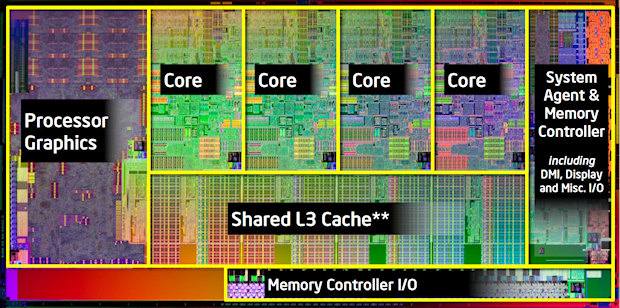
\includegraphics[scale=0.5]{sandy}
  \end{center}
  \caption{
    The figure depicts a quad-core Sandy Bridge microprocessor (or chip). The
    author was unable to locate an image of an octa-core chip.
  }
  \label{fig:p5}
\end{figure}

\subsection{Interconnecting chips to form larger SMPs}

Multiple Sandy Bridge chips can be connected to form larger modules in SMP
configurations. On Vilje, two chips are run in SMP mode on each compute node.
Thus, up to 16 (32) processors share memory.

\subsection{Interconnecting nodes to form a distributed SMP}

Multiple nodes may also be connected to form clusters or distributed SMPs. In
this case, data from one node to another must be passed across a high bandwidth
low-latency switch network. A system based on multiple nodes must therefore be
treated as a distributed memory system (at least globally).

\subsection{Key data for Vilje}

Vilje is based on 1404 nodes. The total number of processors (or cores) is
therefore 22464.

Each node represents a shared memory system with 2 octa-core Sandy Bridge chips
which share 32 GB memory (although a few nodes have 128 GB memory).

Each i7 processor operates at a clock rate of 2.6 GHz. The size of the L1 cache
(3 clocks) is 32 kbyte for data and 32 kbyte for instructions. The size of the
L2 cache (8 clocks) is 256 kbyte, while the size of the shared off-chip L3 cache
is 20 Mbyte.

\section{Programming models}

We have seen that a node (with 16 physical processors) on Vilje represents a
shared memory system where the aggregate memory for the node is globally
available to all the 16 processors. A shared memory programming model (i.e.
OpenMP) can therefore be used within a single node.

If we want to develop programs which can run on more than one node, we need to
use message-passing (i.e. MPI). This is also the programming model we will
emphasize in this course. Even though each node represents a shared memory
system, the message-passing programming model may still be used within a node.
However, the opposite is not true: a shared programming model cannot be used on
a ``pure'' distributed memory system (e.g. on a PC cluster).

Note that a system like Vilje, which represents a shared memory system within a
node, and a distributed memory system across the nodes, can also be programmed
using both programming models within a single program.

\section{Message passing}

Message passing is fundamentally processor-to-processor communication. Only a
local, unique memory is directly available to each processor. Both local and
remote processes must cooperate in order to exchange data and/or synchronize (at
least originally---some changes have been made in the extended version MPI-2).

Note that message-passing is a good way to use distributed shared memory
machines (ccNUMA) because it provides a way to express memory/data locality.

Some of the key advantages of the message-passing model are:
\begin{itemize}
\item {\em Portability}: the model can be used on a collection of
homogeneous or heterogeneous processors connected by a fast or a slow
communication network;
\item {\em Performance}: the approach exploits data locality, as well as the
availability of a large, aggregate memory;
\item {\em Expressiveness}: a limited communcation library suffices for most applications.
\end{itemize}

The Message Passing Interface (MPI) is the de facto standard for message
passing. It is a \emph{library}, not a language. MPI provides efficiency,
portability and functionality. It represents a standardized communcation library
running on a vast number of machines and architectures.
\autoref{fig:message_passing_model} illustrates the message passing model.

The original (1994) MPI-library represents the message passing model where both
the local and remote processes cooperate e.g. via a send and receive
operation. MPI-2 represents an extension of MPI where features like one-sided
messages, parallel I/O, etc. are included.

\begin{figure}
  \centering
  \begin{tikzpicture}[
  proc/.style={shape=circle, draw=darkblue, fill=cadet, thick},
  msg/.style={shape=rectangle, draw=darkblue, fill=cadet, thick, rounded corners=0.5mm},
  env/.style={minimum height=1.7cm, minimum width=1.7cm},
  scale=0.7,
  ]
  \node[proc] (p0) at (0,0) {$P_0$};
  \node[proc] (p1) at (1,3) {$P_1$};
  \node[proc] (p2) at (3,-0.6) {$P_2$};
  \node[proc] (p3) at (6,3.6) {$P_3$};
  \node[msg] (msg) at (4.0, 1.5) {\scriptsize Message};
  \node[msg, env, fill=cadet!55] (env) at (8, -2.0) {};
  \node[msg, very thin] (body) at (8, -1.7) {\scriptsize Body};
  \node[below of=body, node distance=6mm] {\scriptsize Envelope};
  \draw[->, thick] (p2) edge[bend right] node [right] {} (msg);
  \draw[->, thick] (msg) edge[bend right] node [right] {} (p1);
  \draw[->, thick] (env) edge[bend right] node [right] {} (msg);

  \node[msg] (smp) at (-2,-2) {\scriptsize SMP};
  \draw[->, thick] (smp) edge[bend left] node [right] {} (p0);
\end{tikzpicture}

  \caption{
    The message passing model. A number of processes, $P_0, P_1, \ldots,
    P_{n-1}$, are coupled together via a fast or a slow communication network.
    Each process has a local and unique memory/cache, and each process is
    associated with a particular computational task. The individual processes
    must communicate via explicit message passing. A message consists of an
    ``envelope'' which contains sufficient information about whether and when to
    open the message, as well as information regarding how to interpret the
    ``body'' of the message (the actual data). Note that the message is the only
    means of exchanging data between the processes and/or syncronizing the
    processes.
  }
  \label{fig:message_passing_model}
\end{figure}

The MPI operations can be classified in a few types of operations:
\begin{itemize}
\item one-to-one;
\item one-to-all;
\item all-to-one;
\item all-to-all.
\end{itemize}
The first type is also referred to as point-to-point operations (send and
receive), while the last three types are collective operations.

When we here talk about ``all'', we generally mean all processes $P_0, P_1,
\ldots, P_{n-1}$ within a group of $n$ processes. Such a group defines a
\emph{communicator} and the particular process number is referred to as the
\emph{rank} within that communicator. The default is to let all processes be
members of the same (default) communicator. However, it is also possible to have
some of the processes be members of one communicator (or group), while others be
members of a different communicator. In this context, ``all'' means all the
processes \emph{within} a particular communicator.

Finally, the collective operations can be further broken down into the
following categories:
\begin{itemize}
\item data movement (broadcast; gather/scatter);
\item collective computation (max/min; sum; etc.).
\end{itemize}

We will later explain in more detail the various MPI operations. A good way to
learn MPI is by implementing a few simple examples. The whole library contains
about 125 functions. However, as few as 6 may suffice for some problems. You
only need to learn the functions needed for your particular problem. You may not
have to learn the details of the whole library even for advanced applications.

\subsection{An example}

We now discuss a brief example of a program where the MPI library is used. The
program listed below does the following: processor 0 sends a text message
``Hello, world'' to all the other processors. The other processors receive the
message and all processors print out the message together with the their own
process number.

Listings \ref{lst:mpi-hello-c} and \ref{lst:mpi-hello-fortran} show how this is
done in both C and Fortran.

\begin{lstlisting}[style=c, float, caption={Hello world MPI in C.}, label=lst:mpi-hello-c]
  #include <stdio.h>
  #include "mpi.h"

  int main(int argc, char **argv)
  {
    int rank, size, tag, i;
    MPI_Status status;
    char message[20];

    MPI_Init(&argc, &argv);
    MPI_Comm_size(MPI_COMM_WORLD, &size);
    MPI_Comm_rank(MPI_COMM_WORLD, &rank);

    tag = 100;

    if (rank == 0) {
      strcpy(message, "Hello, world");
      for (i = 1; i < size; i++) {
        MPI_Send(message, 13, MPI_CHAR, i,
                 tag, MPI_COMM_WORLD);
      }
    }
    else {
      MPI_Recv(message, 13, MPI_CHAR, 0,
               tag, MPI_COMM_WORLD, &status);
    }

    printf("node %d: %13s\n", rank, message);

    MPI_Finalize();

    return 0;
  }
\end{lstlisting}

\begin{lstlisting}[style=fortran, float, caption={Hello world MPI in Fortran.}, label=lst:mpi-hello-fortran]
  program hello
  include 'mpif.h'

  integer rank, size, ierror, tag, status(MPI_STATUS_SIZE)
  character(12) message

  call MPI_INIT(ierror);
  call MPI_COMM_SIZE(MPI_COMM_WORLD, size, ierror);
  call MPI_COMM_RANK(MPI_COMM_WORLD, rank, ierror);

  tag = 100;

  if (rank .eq. 0) then
    message = 'Hello, world'
    do i=1,size-1
      call MPI_SEND(message, 12, MPI_CHARACTER, i, tag,
                    MPI_COMM_WORLD, ierror)
    enddo
  else
    call MPI_RECV(message, 12 MPI_CHARACTER, 0, tag
                  MPI_COMM_WORLD, status, ierror)
  endif

  print*, 'node', rank, ':', message

  call MPI_Finalize(ierror)
  end
\end{lstlisting}

The output of the C version on the SGI Origin using $P=4$ and $P=8$ processors
is shown in Listings \ref{lst:mpi-hello-4} and \ref{lst:mpi-hello-8}.

\begin{lstlisting}[float, caption={Hello world MPI in C: $4$ processors.}, label=lst:mpi-hello-4]
  node 1: Hello, world
  node 3: Hello, world
  node 2: Hello, world
\end{lstlisting}

\begin{lstlisting}[float, caption={Hello world MPI in C: $8$ processors.}, label=lst:mpi-hello-8]
  node 5: Hello, world
  node 1: Hello, world
  node 7: Hello, world
  node 2: Hello, world
  node 3: Hello, world
  node 6: Hello, world
  node 4: Hello, world
\end{lstlisting}

Let us now comment on some of the statements here. We start with
\begin{lstlisting}[style=c]
  #include <stdio.h>
  #include "mpi.h"
\end{lstlisting}
The first statement is just a standard statement about including the header file
associated with string (character) operations and I/O. The second statement is
required if we want to use the MPI library in our program. In C, we need the
statement
\begin{lstlisting}[style=c]
  #include "mpi.h"
\end{lstlisting}
The equivalent statement in Fortran is
\begin{lstlisting}[style=fortran]
  include 'mpi.f'
\end{lstlisting}
The MPI header file provides basic MPI definitions and MPI data types.

The first MPI statement needs to be:
\begin{lstlisting}[style=c]
  MPI_Init(&argc, &argv);
\end{lstlisting}
This statement should only be called once. The last MPI statement is always
\begin{lstlisting}[style=c]
  MPI_Finalize();
\end{lstlisting}
This statement does not have to be the very last statement in your program, but
it needs to be the last MPI statement. It statement ensures a clean exit.

Note that the command line arguments are passed to the C version of
\texttt{MPI\_Init}. The corresponding Fortran version reads:
\begin{lstlisting}[style=fortran]
  call MPI_INIT(ierror);
\end{lstlisting}
Similar to a standard subroutine call in Fortran, a call to an MPI operation
also starts with \texttt{call}. The parameter \texttt{ierror} is an integer and
will return an error code in case something goes wrong. The C version also
returns an error code. Instead of the statement used in the program listed
above, we could alternatively have written
\begin{lstlisting}[style=c]
  errorcode = MPI_Init(&argc, &argv);
\end{lstlisting}
In this case, the variable \texttt{errorcode} (an integer) will contain an error
code if something goes wrong.

In general, any MPI statement in C has the format
\begin{lstlisting}[style=c]
  errorcode = MPI_Xxxxx(parameters...);
\end{lstlisting}
or simply
\begin{lstlisting}[style=c]
  MPI_Xxxxx(parameters...);
\end{lstlisting}
The particular MPI operation is given by ``Xxxxx'' where the name of the operation
always starts with a capital letter and the remaining letters are lower-case.
The number and type of parameters vary from operation to operation. For example,
\texttt{MPI\_Finalize} does not have any parameters at all.

In Fortran, any MPI statement has the format.
\begin{lstlisting}[style=c]
  call MPI_XXXXX(parameters..., ierror)
\end{lstlisting}
where the parameter \emph{ierror} returns an error code. Note that the name of
the particular MPI operation is always in capital letters.

The next two statements after the initialization of MPI are:
\begin{lstlisting}[style=c]
  MPI_Comm_size (MPI_COMM_WORLD, &size);
  MPI_Comm_rank (MPI_COMM_WORLD, &rank);
\end{lstlisting}
The first of these statements returns the total number of MPI processes, while
the second one returns the individual process number (the ``rank''). More
precisely, the process number is stored in the location pointed to by the second
argument. \texttt{MPI\_COMM\_WORLD} is the default name of the communicator (the
``univertse'') and which include all the processes. This can be changed in order
to create several separate ``universes.''

Note that the program listed in this example runs separately and independently
on every processor on a multiprocessor. We also refer to this as SPMD -
\emph{Single Program Multiple Data}. All the problems we will study in this
course will be of this type: the program running on each processor will be the
same for all the processors. However, the data each processor will operate on
will typically be different. The synchronization of the program will be implicit
via the MPI operations. We will return to this issue later.

When this program runs on a particular processor, the program does not
automatically know how many other processors are involved; this issue is taken
care of by the MPI operation \texttt{MPI\_Comm\_size}. In the multiprocess
context, the program running on an individual processor does not automatically
know what its associated process number is (who am I?); this issue is taken care
of by the MPI operation \texttt{MPI\_Comm\_rank}.

Let us now proceed to the statements
\begin{lstlisting}[style=c]
  if (rank == 0) {
    strcpy (message, "Hello, world");
\end{lstlisting}
The if-statement will only be true for one of the processes, namely, the process
with process number 0. This is also referred to as the ``root'' process. On the
root process, the string ``Hello, world'' is copied into the string variable
\texttt{message}.

For all the other processes, the if-statement will not be true, and the program
execution will move on to the MPI statement \texttt{MPI\_Recv}. This means that
all of the other processes will be waiting for the root process to send them
data. The root process sends data to the other processes in the loop
\begin{lstlisting}[style=c]
  for (i=1; i < size; i++) {
    MPI_Send(message, 13, MPI_CHAR, i,
             tag, MPI_COMM_WORLD);
  }
\end{lstlisting}
Several comments are in order here. First, note that the root process sends out
the same message (string) to all the other processes. This is done in a loop.
However, note that this loop corresponds to a \emph{sequential} execution
meaning that a message will be sent to process $1$ before process $2$ etc.

Let us now discuss the particular format in the parameter list for the operation
\texttt{MPI\_Send}. The general format for this operation is
\begin{lstlisting}[style=c]
  MPI_Send(start, count, datatype, dest, tag, comm);
\end{lstlisting}
The first three parameters (start, count, datatype) represent \emph{the data},
while the last three parameters (dest, tag, comm) represent \emph{the envelope};
see \autoref{fig:message_passing_model}.

We now explain all these parameters in some more detail.
\begin{itemize}
\item \emph{start}: initial address of the send buffer
\item \emph{count}: number of elements sent (of type \texttt{datatype})
\item \emph{datatype}: e.g. \texttt{MPI\_INT}, \texttt{MPI\_FLOAT}, \texttt{MPI\_CHAR} etc.
\item \emph{dest}: destination process (integer)
\item \emph{tag}: integer message identifier (e.g., \texttt{MPI\_ANY\_TAG})
\item \emph{comm}: an ordered group of communication processes (same for send
  and receive)
\end{itemize}

Only the root process sends a message. All the other processes are waiting to
receive a message. This is expressed by the MPI operation \texttt{MPI\_Recv}.
The general format for this operation is
\begin{lstlisting}[style=c]
  MPI_Recv(start, count, datatype, source, tag, comm, &status);
\end{lstlisting}
The first three parameters (start, count, datatype) represent \emph{the data},
while the last three parameters (dest, tag, comm, status) represent \emph{the
envelope}; again, see \autoref{fig:message_passing_model}.

Most of the parameters are similar to the MPI\_Send operation:
\begin{itemize}
\item \emph{start}: initial address of the receive buffer
\item \emph{count}: number of elements sent (of type \emph{datatype})
\item \emph{datatype}: e.g. \texttt{MPI\_INT}, \texttt{MPI\_FLOAT}, \texttt{MPI\_CHAR} etc.
\item \emph{source}: source process (integer), i.e., the process sending the message
\item \emph{tag}: integer message identifier (e.g., \texttt{MPI\_ANY\_TAG})
\item \emph{comm}: an ordered group of communication processes (same for send and receive)
\item \emph{status}: a structure providing information on the completed communication
\end{itemize}

Note that in the small example program, an explicit source is given, namely, the
root process. Alternatively, we could have used \texttt{MPI\_ANY\_SOURCE} since
each process in receive mode only expects one message. Similarly, we note that
the ``tag'' is explicitly given. Alternatively, we could have used
\texttt{MPI\_ANY\_TAG} since this parameter is not critical in our case.

One additional comment regarding the send and receive statements. This is an
example of point-to-point communication. There exists several versions of send
and receive. The type used here is called \emph{blocking} send and receive. This
means that the program running on the root processor cannot proceed until each
message has been safely sent and the send buffer can be safely used again.
Similarly, the program running on each of the other processors cannot proceed
until the expected message has been received in the receive buffer.

Let us now comment on the parameter \emph{count} used in the send and receive
statements. In the C version, the count parameter is set equal to 13, while it
is 12 in the Fortran version. The reason for this is that the \texttt{strcpy}
function in C will append \texttt{\textbackslash 0} (the null character) at the
end of the message. This is a symbol which indicates the end of the string. Even
though ``Hello, world'' comprises 12 letters (one byte per letter), the message
buffer in C requires 13 bytes of memory.

The parameter ``datatype'' in the send and receive operations has to be the same.
In this case, the type is \texttt{MPI\_CHAR} (in Fortran the corresponding data
type is called \texttt{MPI\_CHARACTER}). This is one of several predefined data
types. Other important ones include \texttt{MPI\_DOUBLE} and \texttt{MPI\_INT}.

Finally, note that the output from the programs is not in a sequential order.
The order may also change if we run the program over again.
